% Shared standalone design for the editable figure reconstructions.
\documentclass[tikz,border=5pt,10pt]{standalone}
\usepackage[T1]{fontenc}
\usepackage[utf8]{inputenc}
\usepackage{newpxtext,newpxmath}
\usepackage[scaled=.94]{sourcesanspro}
\usepackage{pgfplots}
\pgfplotsset{compat=1.18}
\usetikzlibrary{arrows.meta,calc,positioning,decorations.pathreplacing,
  decorations.markings,patterns,matrix,shapes.geometric,fit,backgrounds,
  intersections,angles,quotes}
\definecolor{ink}{HTML}{203746}
\definecolor{accent}{HTML}{146C78}
\definecolor{muted}{HTML}{667780}
\definecolor{signalred}{HTML}{B94B44}
\color{ink}
\tikzset{>=Latex,line width=.8pt,
  every node/.style={font=\small},
  axis/.style={->,draw=muted,line width=.5pt},
  guide/.style={draw=muted,dashed,line width=.45pt},
  curve/.style={draw=accent,line width=1pt},
  marker/.style={circle,fill=accent,inner sep=1.5pt},
  labelbox/.style={fill=white,inner sep=2pt}}

\begin{document}
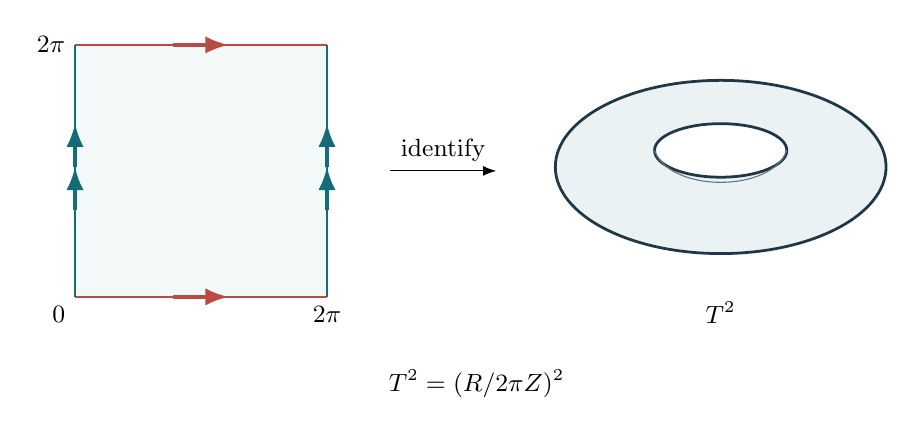
\begin{tikzpicture}[x=1cm,y=1cm]
\fill[accent!5] (0,0) rectangle(3.2,3.2);
\draw[signalred,line width=1pt] (0,0)--(3.2,0) (0,3.2)--(3.2,3.2);
\draw[accent,line width=1pt] (0,0)--(0,3.2) (3.2,0)--(3.2,3.2);
\foreach \y in {0,3.2} {\draw[->,signalred,line width=1.2pt] (1.25,\y)--(1.95,\y);}
\foreach \x in {0,3.2} {\draw[->,accent,line width=1.2pt] (\x,1.1)--(\x,1.65);\draw[->,accent,line width=1.2pt] (\x,1.65)--(\x,2.2);}
\node[below left] at (0,0) {$0$};\node[below] at (3.2,0) {$2\pi$};\node[left] at (0,3.2) {$2\pi$};
\draw[->] (4,1.6)--node[above] {identify}(5.35,1.6);
\path[fill=accent!9,draw=ink,line width=1pt,even odd rule] (8.2,1.65) ellipse(2.1 and 1.1) (8.2,1.86) ellipse(.84 and .34);
\draw[muted] (7.36,1.86)..controls(7.55,1.32)and(8.85,1.32)..(9.04,1.86);
\node at (8.2,-.2) {$\mathbb T^2$};
\node at (5.1,-1.1) {$\mathbb T^2=(\mathbb R/2\pi\mathbb Z)^2$};
\end{tikzpicture}
\end{document}
